% !TeX encoding = UTF-8
\section{Grundlagen}
\label{Grundlagen}
Dieses Kapitel führt die verwendeten Algorithmen und Berechnungen ein.\\
Mit dem A*-Algorithmus wurde schon in den 60er Jahren ein Werkzeug für die Pfadplannung von Robotern eingeführt[TODO Literaturverweis]. Pfadplannung bedeutet hier, dass ein Roboter mit festgelegten kinematischen Einschränkungen in einer bestimmten, definierten Umgebung von einem Startzustand zu einem Zielzustand mithilfe von Steuerungseingaben gelangen kann, ohne die physikalischen Gesetze und die der Umgebung (keine Kollision mit Hindernissen) zu verletzen. Der A*-Algorithmus löst dieses Problem mit vielen Einschränkungen, indem er in einem Graphen den kürzesten Weg zwischen zwei Knoten findet. Allerdings benötigt A* diesen Graphen zur Berechnung des Weges und ist aufgrund des hohen Speicherplatzbedürfnisses für \textit{hochdimensionale Probleme}, d.h. für Probleme mit den oben genannten Einschränkungen, nicht geeignet[TODO Zitat].\\
In nachfolgender Zeit wurden \textit{randomisierte Algorithmen} [TODO weitere Erklärungen zu randomisierten Alg und deren Vorteile] entwickelt, die diese Probleme nicht mehr hatten, wie der \textit{randomized potential field} Algorithmus \citep{BaLa91} und der \textit{probalistic roadmap} Algorithmus \citep{AmWu96}. Doch auch diese waren nicht allgemein auf \textit{nonholonomic Robots} anwendbar und lösten oft nur spezifische Probleme unter ganz bestimmten Bedingungen. Der Erfolg des \textit{randomized potential field} Algorithmus beispielsweise hing stark von der Wahl einer passenden Heuristik ab \citep[vgl. Kap 3.4][]{BaLa91}. Während sich bei einfachen Ausgangsbedingungen die Heuristik noch einfach finden lies, wurde dies bei komplexen, dynamischen Umgebungen mit Hindernissen, physikalischen und kinematischen Bedingungen zu einer großen Herausforderung. \\
1998 schließlich führte Steven LaValle den \textit{RRT}-Algorithmus ein, der die oben genannten Einschränkungen umgehen sollte.

\subsection{RRT}
\label{RRT}
LaValle erkannte die sowohl die Vorteile von randomisierten Algorithmen als auch die Nachteile der existierenden Algorithmen \citep[vlg. Kap 1][]{Lav98}. Insbesondere störten ihn die fehlende Skalierbarkeit vieler Algorithmen in komplexere Umgebungen, da diese Algorithmen damit nur unter gewissen Vorbedingungen effizient einsetzbar waren. Der \textit{probalistic roadmap} Algorithmus \citep{AmWu96} beispielsweise [TODO] .\\
Bei der Entwicklung von \textit{RRT} wurde deshalb viel Wert auf Einfachheit, Allgemeingültigkeit und damit auf Skalierbarkeit gelegt \citep[vlg. Kap 3][]{Lav98}. Bevor wir jedoch genauer auf die Vorteile des Algorithmus eingehen und warum dieser hier gewählt wurde, folgt jetzt erstmal eine kurze Erklärung der Funktionsweise. RRT baut einen Baum auf, indem zufällig gewählte Punkte unter Berücksichtigung einer Metrik verbunden werden. Der Algorithmus mit dem \textit{RRT} $T$ mit den Eingabeparametern Größe $K$, Metrik $M$, Bewegungsfunktion $u$, und Startzustand \verb|x_init|  funktioniert folgendermaßen:

\subsubsection{Funktionsweise RRT}
[TODO in Quellcode Literaturverweis]
\lstset{language=Pascal, stepnumber=1, numbers=left}
\begin{lstlisting}
BUILD_RRT(K, M, u, x_init)
	T.init (x_init)
	for k=1 to K do
		x_rand = RANDOM_STATE();
		EXTEND(T, x_rand);
	Return T;
\end{lstlisting}
\begin{lstlisting}
EXTEND(T, x)
	x_near = NEAREST_NEIGHBOR(x, T, M);
	x_new = project(x, x_near, u);
	if (Collisionfree(x_new, x_near, u) then
		T.add_vertex(x_new);
		T.add_egde(x_near, x_new, u_new);
		Return Extended;
	else
		Return Trapped;
\end{lstlisting}

Der Baum wird anfangs mit dem Startzustand \verb|x_init| initialisiert. Anschließend wird in $K$ Iterationen der Baum $T$ aufgebaut, indem mit \verb|x_rand| ein zufälliger Punkt ausgewählt und mit \verb|EXTEND(T, x_rand)| dem Baum hinzugefügt wird. \\
Die Funktion \verb|EXTEND(T, x)| ermittelt zunächst mithilfe der Metrik $M$ den nächsten Nachbar von $x$. Diese Metrik kann von einer einfachen euklidischen Distanz bis hin zur komplexen Einberechnung verschiedener kinetmatischer Bedingungen alles beinhalten. Die hier verwendete Metrik wird später noch in Kapitel \ref{Metrik} beleuchtet. \\
Ist der nächste Nachbar \verb|x_near| gefunden, wird von diesem aus mit \verb|project(x, x_near, u)|  ein Schritt der Länge  $\epsilon$ in Richtung x durchgeführt und an dieser Stelle der neue Knoten \verb|x_new| erzeugt. 
\begin{figure}
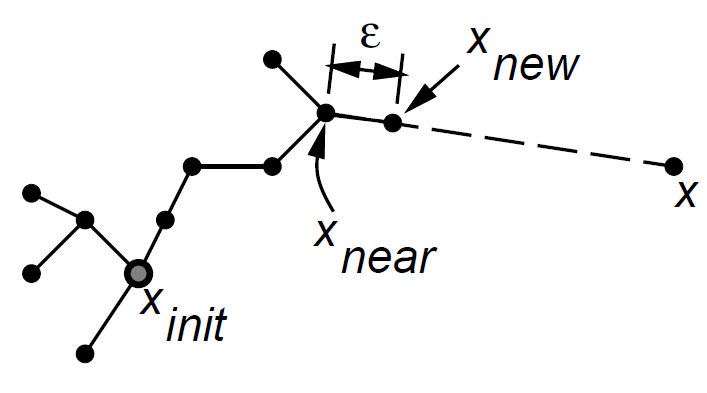
\includegraphics[scale=1]{Bilder/Extend.png} 
\caption{Die EXTEND Funktion \citep{Lav00} }
\label{fig3}
\end{figure} \\
Nun wird mit \verb|Collsionfree(x_new, x_near, u)| überprüft, ob \verb|x_new| oder die Bewegung $u$ zu \verb|x_new| hin mit Hindernissen kollidiert oder diesen zu Nahe kommt. Falls dies nicht der Fall ist, werden sowohl der neu entstandene Knoten \verb|x_new| als auch die Kante von \verb|x_near| zu \verb|x_new| dem Baum $T$ hinzugefügt. \\
Falls  \verb|x_new| oder die Bewegung u zu  \verb|x_new| mit Hindernissen kollidiert oder diesen zu Nahe kommt, wird der Knoten  \verb|x_new| verworfen und die Funktion \verb|EXTEND(T,x)| beendet.\\

\subsubsection{Vor- und Nachteile von RRT}
Die Rapidly-Exploring Random Trees haben einige Eigenschaften, die für Bewegungsplanung von Robotern von großem Vorteil sind, wie LaValle in  [TODO Literarur LaValle Kap 3] schreibt:
\begin{enumerate}
\item Ein \textit{RRT} breitet sich sehr schnell in unerforschte Bereiche des Statusraums aus. Dadurch können Pfade schnell gefunden werden und es wird schnell eine mögliche (wenn auch nicht optimale) Lösung gefunden.
\item Die Verteilung der Knoten im Baum entspricht der Verteilung, wie diese Knoten erzeugt wurden; dies führt zu konsistentem Verhalten. Unter anderem kann dadurch das Wachstum des Baumes in eine bestimmte Richtung gesteuert werden (z.B. zum Ziel hin)
\item Ein \textit{RRT} ist probabilistisch vollständig, das heißt mit zunehmender Laufzeit konvergiert die Wahrscheinlichkeit, keinen Pfad zum Ziel zu finden, gegen null
\item Ein \textit{RRT} ist sowohl einfach zu implementieren als auch einfach in der Analyse, was es ermöglicht die Performance einfach zu analysieren und zu verbessern
\item Ein \textit{RRT} ist immer mit sich selbst verbunden, und das bei einer minimalen Kantenanzahl
\item Ein \textit{RRT} kann als Pfadplanungsmodul interpretiert werden, was die Kombination mit anderen Werkzeugen zur Bewegungsplanung möglich macht
\end{enumerate}
Leider existieren neben den oben genannten Vorteilen auch etliche Nachteile. Eines der größten ist, dass ein \textit{RRT} nicht den optimalen Pfad zurückliefert, da einmal gesetzte Knoten ihren Vaterknoten nicht mehr ändern können. Dadurch kann, auch wenn eine bessere Knotenfolge vom Start zum Ziel bestehen würde, diese nicht ausgewählt werden. \\
\begin{figure}
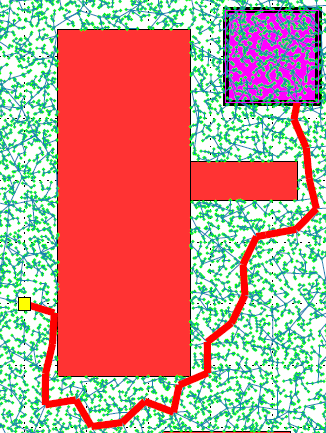
\includegraphics[scale=1]{Bilder/rrt_path.png} 
\caption{Ausschnitt eines RRT Graphs mit 20.000 Knoten \citep{KaFra10} }
\end{figure}
Deshalb wurde von Sertac Karaman und Emilio Frazzoli aufbauend auf \textit{RRTs} der Algorithmus\textit{ RRT*} eingeführt, welcher diesen Nachteil ausgleicht.
\subsection{RRT*}
\label{RRT*}
Im Gegensatz zu einem \textit{RRT} führt ein \textit{RRT*} die zwei folgenden Neuerungen ein:
\begin{enumerate}
\item Auswahl eines passenden Vaterknotens bei Hinzufügen des Knotens zum Baum
\item Neuverknüpfung des Baumes
\end{enumerate}

Diese Neuerungen resultieren in einer veränderten \verb|EXTEND(T,x)| Funktion, siehe \citep{KaFra10}.
\subsubsection{Funktionsweise RRT*}
\begin{lstlisting}
EXTEND(T,x)
	x_nearest = NEAREST_NEIGHBORS(x, T, M);
	x_new = project(x, x_nearest, u);
	if (Collisionfree(x_new, x_near, u) then
		T.add_vertex(x_new);
		x_min= x_nearest;
		c_min = x_nearest.cost + cost(x_nearest, x_new);
		X_NEAR = NEAR_NEIGHBORS(x, T, r);
		foreach x_near in X_NEAR do
			if Collisionfree(x_near, x_new) && x_near.cost + cost(x_near, x_new) < c_min then
				x_min = x_near;
				c_min = x_near.cost + cost(x_near, x_new);
		T.add_egde(x_min, x_new);
		foreach x_near in X_NEAR do
			if Collsionfree(x_new, x_near) && x_new.cost + cost(x_new, x_near) < x_near.cost then
				T.del_edge(x_near_parent, x_near);
				T.add_edge(x_new, x_near);
		Return Extended;
	else
		Return Trapped;
\end{lstlisting}

Während wie beim Erstellen eines \textit{RRT} auch bei \textit{RRT*} zuerst der nächste Nachbar als Vaterknoten festgelegt wird, folgt daraufhin eine Speicherung der nächsten Nachbarn von \verb|x_new| in einem gewissen Radius $r$ in der Liste \verb|X_NEAR|. 
Es wird \verb|x_min| als der Abstand zum nächsten Knoten gesetzt. Die Funktion \verb|x_nearest.cost| liefert die Kosten, um vom Startknoten zu \verb|x_nearest| zu kommen, zurück, während die Funktion \verb|cost(x_nearest, x_new| die Kosten des Pfades von \verb|x_nearest| zu \verb|x_new| berechnet. Als vorläufiger Startwert beinhaltet \verb|c_min| demnach die Kosten, um vom Startknoten aus zu \verb|x_new| zu kommen. \\
Die Liste \verb|X_NEAR| wird nun durchiteriert, um den besten Nachbarn, also den mit den geringsten Kosten, für \verb|x_new| zu finden. Dazu wird jedesmal verglichen, ob (sofern \verb|x_new| überhaupt durch \verb|x_near| erreichbar ist) die Kosten, um \verb|x_new| zu erreichen, geringer sind als die bisher geringsten Kosten. Wurde die Liste durchiteriert, wird der beste gefundene Nachbar für \verb|x_new| als Vaterknoten gesetzt, also eine Kante zwischen \verb|x_new| und \verb|x_near| gezogen. \\
Nachdem so ein Pfad vom Startknoten zu \verb|x_new| gebildet wurde, wird überprüft, für welche Knoten in der Liste \verb|X_NEAR| wiederum der in diesem Schritt hinzugefügte Knoten \verb|x_new| die Gesamtkosten vom Startknoten aus verringern würde. Dazu wird wieder \verb|X_NEAR| durchiteriert und bei allen Knoten \verb|x_near|, wo der Weg über \verb|x_new| geringere Kosten verursacht, \verb|x_new| als Vaterknoten gesetzt.
\subsubsection{Vor- und Nachteile RRT*}
Der erste Unterschied zu einem \textit{RRT} ist, dass nicht der nächste Nachbar als Vaterknoten gesetzt wird, sondern der mit den besten Kosten. Je nach Wahl des Radius $r$ kann hier einiges an "Umweg" gespart werden. \\
Der Hauptunterschied ist jedoch die Neuverknüpfung bereits bestehender Knoten über \verb|x_new|. Ein Nachteil des \textit{RRTs} war auch, dass Knoten, die aus bereits gut mit Knoten gefüllten Regionen neu hinzugefügt wurden den Baum nicht wirklich bereichert hatten. Dies ändert sich nun, denn jeder von Knoten umgebene neu hinzugefügte Knoten verbessert die Kosten der meisten Knoten, sofern sie durch \verb|x_new| besser erreichbar ist. Dies führt sogar soweit, dass ein \textit{RRT*} asymptotisch optimal ist, d.h. bei genügend langer Laufzeit der Pfad zum Optimum konvergiert.[TODO Literaturverweis]. Je nach Art der Kostfunktion kann der RRT* auch mit bestimmten Eigenschaften ausgestattet werden, z.B. präferiertes Wachsen in bestimmte Richtungen.
\subsection{Nicht-holonomische Einschränkungen}
Leider ist dieser Algorithmus so nicht eins zu eins auf ein Auto umsetzbar, da dieses bestimmten kinematischen Bedingungen unterworfen ist. Es kann sich zum Beispiel nicht in jede beliebige Richtung bewegen (z.B. seitlich) und hat abhängig vom Lenkradius gewisse Punkte, die nicht in einem Schritt erreichbar sind. Wie die Einschränkungen genau aussehen, welche Rahmenbedingungen an Hardware und Software gegeben waren und inwieweit der RRT*-Algorithmus angepasst werden musste, behandelt das nächste Kapitel.